\documentclass[aspectratio=169,10pt]{beamer}

% --- Typography & Core Setup ---
\usepackage[utf8]{inputenc}
\usepackage[T1]{fontenc}
\usepackage{lmodern}
\usepackage{amsmath,amssymb}
\usepackage{booktabs}
\usepackage{tabularx}
\usepackage{graphicx}
\usepackage{tikz}
\usetikzlibrary{shapes.geometric,arrows.meta,positioning,calc,fit}

% Image search paths
\graphicspath{{data/reports/}{../data/reports/}{./}}

% --- Soothing, Eye-Friendly Color Palette (Nordic Sage & Warm Linen) ---
\definecolor{CanvasBg}{RGB}{248, 246, 240}      % Soft Warm Cream
\definecolor{DeepCharcoal}{RGB}{40, 44, 48}     % Dark Charcoal for readable text
\definecolor{SageGreen}{RGB}{46, 89, 70}        % Calming Forest Sage (Primary)
\definecolor{MutedAmber}{RGB}{175, 110, 65}     % Gentle Terracotta / Ochre (Accent)
\definecolor{CardBg}{RGB}{240, 237, 229}        % Light Linen for cards
\definecolor{CardBorder}{RGB}{215, 210, 200}    % Muted Stone Border
\definecolor{SlateText}{RGB}{105, 110, 115}     % Soft Gray for captions
\definecolor{BoxAccent}{RGB}{232, 238, 233}     % Very light sage tint for diagram nodes

% Apply Beamer Colors
\setbeamercolor{background canvas}{bg=CanvasBg}
\setbeamercolor{normal text}{fg=DeepCharcoal}
\setbeamercolor{title}{fg=SageGreen}
\setbeamercolor{frametitle}{fg=SageGreen}
\setbeamercolor{structure}{fg=SageGreen}
\setbeamercolor{item}{fg=SageGreen}
\setbeamercolor{block title}{bg=SageGreen,fg=white}
\setbeamercolor{block body}{bg=CardBg,fg=DeepCharcoal}

% Clean slide headers without harsh lines
\setbeamertemplate{navigation symbols}{}
\setbeamertemplate{frametitle}{
    \vspace{0.35cm}
    {\large\textbf{\insertframetitle}}
    \par\vskip 3pt
    {\color{SageGreen!40}\rule{\textwidth}{0.6pt}}
}

% Minimal page numbering
\setbeamertemplate{footline}{
    \hfill
    \footnotesize\color{SlateText}\insertframenumber{} / \inserttotalframenumber\hspace*{0.6cm}\vskip0.35cm
}

% TikZ Common Styles for Neat Block Diagrams
\tikzset{
    block/.style={
        rectangle,
        draw=SageGreen,
        fill=BoxAccent,
        thick,
        rounded corners=3pt,
        text centered,
        minimum height=0.75cm,
        font=\scriptsize\bfseries,
        text=DeepCharcoal
    },
    priorblock/.style={
        rectangle,
        draw=MutedAmber,
        fill=CardBg,
        thick,
        rounded corners=3pt,
        text centered,
        minimum height=0.75cm,
        font=\scriptsize\bfseries,
        text=DeepCharcoal
    },
    arrow/.style={
        -{Latex[length=2.5mm]},
        thick,
        SageGreen
    },
    dashedarrow/.style={
        -{Latex[length=2.5mm]},
        dashed,
        thick,
        MutedAmber
    }
}

% --- Metadata ---
\title{\textbf{MasterRTL+: Enhancing Presynthesis PPA Estimation}}
\subtitle{Architectural Upgrades \& Hybrid Physics Priors for Chip Design}
\author{Chopperla Santosh}
\date{\today}

\begin{document}

% -------------------------------------------------------------
% Slide 1: Opening Slide (Personal Details & Domain)
% -------------------------------------------------------------
\begin{frame}[plain]
    \vspace{1.4cm}
    {\huge \textbf{\color{SageGreen}MasterRTL+}}\\[0.25cm]
    {\large \color{DeepCharcoal}Enhanced Presynthesis PPA Estimation for RTL Designs}\\[0.4cm]
    {\color{SageGreen!30}\rule{0.6\textwidth}{1.0pt}}\\[0.7cm]

    \small
    \textbf{Name}: Chopperla Santosh\\[0.15cm]
    \textbf{Roll Number}: S20240020279\\[0.15cm]
    \textbf{Project Domain}: ML in VLSI
\end{frame}

% -------------------------------------------------------------
% Slide 2: The Core Problem: Synthesis Turnaround Time
% -------------------------------------------------------------
\begin{frame}{The Problem: Slow Feedback in Chip Design}
    \vspace{0.1cm}
    \begin{columns}[T]
        \begin{column}{0.48\textwidth}
            \begin{block}{\centering Traditional Industry Flow}
                \footnotesize
                \begin{itemize}
                    \item Commercial synthesis converts code to gates.
                    \item \textbf{Bottleneck}: Takes \textbf{hours or days} per design.
                    \item Slow feedback delays chip architectural choices.
                \end{itemize}
            \end{block}
        \end{column}
        \begin{column}{0.48\textwidth}
            \begin{block}{\centering Presynthesis Machine Learning}
                \footnotesize
                \begin{itemize}
                    \item Evaluates code directly in \textbf{under 1 second}.
                    \item Bypasses lengthy commercial synthesis runs.
                    \item Provides instant feedback during design exploration.
                \end{itemize}
            \end{block}
        \end{column}
    \end{columns}
    \vfill
    \begin{center}
        \small
        \textbf{Commercial EDA}: Code $\xrightarrow{\quad\textbf{Hours to Days}\quad}$ Synthesis $\to$ PPA Metrics\\
        \textbf{MasterRTL+}: Code $\xrightarrow{\quad\mathbf{< 1.0\textbf{ Second}}\quad}$ Fast ML Engine $\to$ PPA Metrics
    \end{center}
\end{frame}

% -------------------------------------------------------------
% Slide 3: Chip Design Primer: Understanding PPA
% -------------------------------------------------------------
\begin{frame}{Chip Design Primer: Understanding PPA}
    Every silicon chip is judged by three fundamental physical metrics:
    \vspace{0.2cm}
    \begin{columns}[T]
        \begin{column}{0.31\textwidth}
            \begin{block}{\centering 1. Performance}
                \footnotesize
                \begin{itemize}
                    \item Clock deadline margin
                    \item Measured via \textbf{Slack} (ns)
                    \item Negative = timing failure
                \end{itemize}
            \end{block}
        \end{column}
        \begin{column}{0.31\textwidth}
            \begin{block}{\centering 2. Power}
                \footnotesize
                \begin{itemize}
                    \item Energy consumed (mW)
                    \item \textbf{Dynamic}: Signal switching
                    \item \textbf{Static}: Idle leakage
                \end{itemize}
            \end{block}
        \end{column}
        \begin{column}{0.31\textwidth}
            \begin{block}{\centering 3. Silicon Area}
                \footnotesize
                \begin{itemize}
                    \item Chip footprint ($\mu\text{m}^2$)
                    \item \textbf{Sequential}: Flip-flops
                    \item \textbf{Combinational}: Logic gates
                \end{itemize}
            \end{block}
        \end{column}
    \end{columns}
\end{frame}

% -------------------------------------------------------------
% Slide 4: End-to-End Pipeline: How the Architecture Works
% -------------------------------------------------------------
\begin{frame}{End-to-End Architecture: The 4-Stage Pipeline}
    \centering
    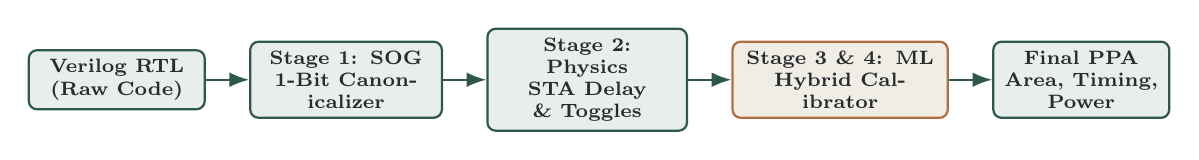
\begin{tikzpicture}[node distance=0.45cm and 0.55cm, auto]
        \node[block, text width=2.0cm] (rtl) {Verilog RTL\\(Raw Code)};
        \node[block, text width=2.2cm, right=of rtl] (sog) {Stage 1: SOG\\1-Bit Canonicalizer};
        \node[block, text width=2.3cm, right=of sog] (phys) {Stage 2: Physics\\STA Delay \& Toggles};
        \node[priorblock, text width=2.5cm, right=of phys] (ml) {Stage 3 \& 4: ML\\Hybrid Calibrator};
        \node[block, text width=2.0cm, right=of ml] (ppa) {Final PPA\\Area, Timing, Power};

        \draw[arrow] (rtl) -- (sog);
        \draw[arrow] (sog) -- (phys);
        \draw[arrow] (phys) -- (ml);
        \draw[arrow] (ml) -- (ppa);
    \end{tikzpicture}

    \vspace{0.4cm}
    \begin{columns}[T]
        \begin{column}{0.48\textwidth}
            \begin{block}{\centering Front-End Canonicalization}
                \footnotesize
                \begin{itemize}
                    \item Unrolls multi-bit vectors into 1-bit primitives.
                    \item Extracts wire loads and signal toggle probabilities.
                \end{itemize}
            \end{block}
        \end{column}
        \begin{column}{0.48\textwidth}
            \begin{block}{\centering Physics-Guided ML Calibration}
                \footnotesize
                \begin{itemize}
                    \item Stage A: Linear prior locks in physical circuit scaling.
                    \item Stage B: XGBoost residual booster refines parasitics.
                \end{itemize}
            \end{block}
        \end{column}
    \end{columns}
\end{frame}

% -------------------------------------------------------------
% Slide 5: Inside Stage 1: The Simple Operator Graph (SOG)
% -------------------------------------------------------------
\begin{frame}{Stage 1: The Simple Operator Graph (SOG)}
    \begin{columns}[c]
        \begin{column}{0.50\textwidth}
            \centering
            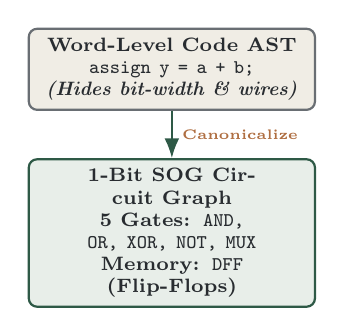
\begin{tikzpicture}[node distance=0.4cm and 0.5cm, auto]
                \node[block, text width=3.4cm, fill=CardBg, draw=SlateText] (ast) {Word-Level Code AST\\\texttt{assign y = a + b;}\\\textit{(Hides bit-width \& wires)}};
                \node[block, text width=3.4cm, below=0.6cm of ast] (sog) {1-Bit SOG Circuit Graph\\5 Gates: \texttt{AND, OR, XOR, NOT, MUX}\\Memory: \texttt{DFF} (Flip-Flops)};
                \draw[arrow] (ast) -- node[right, font=\tiny\bfseries, text=MutedAmber]{Canonicalize} (sog);
            \end{tikzpicture}
        \end{column}
        \begin{column}{0.48\textwidth}
            \begin{block}{\centering Why 1-Bit SOG is Superior}
                \footnotesize
                \begin{itemize}
                    \item An 8-bit adder physically expands into dozens of 1-bit gates and wires.
                    \item Syntax trees hide real wire counts and logic depth ($R \approx 0.82$).
                    \item SOG exposes exact fan-out and wire loads ($\mathbf{R \approx 0.99}$).
                \end{itemize}
            \end{block}
        \end{column}
    \end{columns}
    \vfill
    \begin{center}
        \small\textit{Hardware operates on physical wires, not abstract code syntax.}
    \end{center}
\end{frame}

% -------------------------------------------------------------
% Slide 6: Area Architecture & Our Hybrid Prior Upgrade
% -------------------------------------------------------------
\begin{frame}{Area Architecture: Hybrid Linear Prior + Residuals}
    \centering
    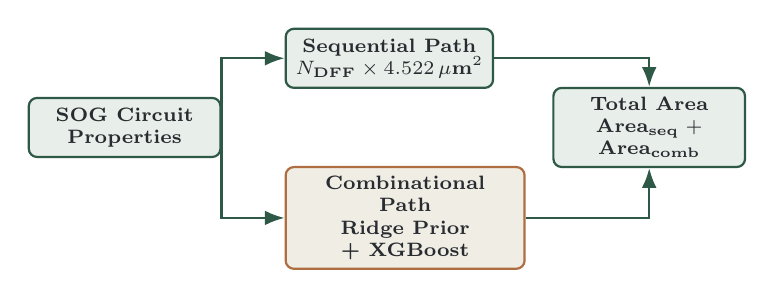
\begin{tikzpicture}[node distance=0.4cm and 0.5cm, auto]
        \node[block, text width=2.2cm] (in) {SOG Circuit\\Properties};
        
        \node[block, text width=2.4cm, above right=0.1cm and 0.8cm of in] (seq) {Sequential Path\\$N_{\text{DFF}} \times 4.522\,\mu\text{m}^2$};
        
        \node[priorblock, text width=2.8cm, below right=0.1cm and 0.8cm of in] (comb) {Combinational Path\\Ridge Prior + XGBoost};
        
        \node[block, text width=2.2cm, right=1.0cm of in, xshift=3.2cm] (sum) {Total Area\\$\text{Area}_{\text{seq}} + \text{Area}_{\text{comb}}$};

        \draw[arrow] (in.east) |- (seq.west);
        \draw[arrow] (in.east) |- (comb.west);
        \draw[arrow] (seq.east) -| (sum.north);
        \draw[arrow] (comb.east) -| (sum.south);
    \end{tikzpicture}

    \vspace{0.3cm}
    \begin{columns}[T]
        \begin{column}{0.48\textwidth}
            \begin{block}{\centering Original Paper Limitation}
                \footnotesize
                \begin{itemize}
                    \item Pure deep XGBoost regressor (depth 12).
                    \item Predictions plateaued on large designs ($\mathbf{5.21\%}$ error).
                \end{itemize}
            \end{block}
        </column}
        \begin{column}{0.48\textwidth}
            \begin{block}{\centering Our Upgraded Solution}
                \footnotesize
                \begin{itemize}
                    \item Ridge prior locks in exact standard cell gate scaling.
                    \item XGBoost refines non-linear wire routing congestion.
                    \item \textbf{Result: Error dropped to 1.80\% ($R = 1.00$)}.
                \end{itemize}
            \end{block}
        \end{column}
    \end{columns}
\end{frame}

% -------------------------------------------------------------
% Slide 7: Timing Architecture & Our Endpoint Prior Upgrade
% -------------------------------------------------------------
\begin{frame}{Timing Architecture: Analytical Endpoint Priors}
    \centering
    
\begin{tikzpicture}[node distance=0.4cm and 0.6cm, auto]
        \node[block, text width=1.9cm] (sog) {SOG DAG\\Circuit Graph};
        \node[block, text width=2.1cm, right=of sog] (sta) {STA Traversal\\Critical Paths};
        \node[block, text width=2.1cm, right=of sta] (rf) {Path Model\\Random Forest};
        \node[priorblock, text width=2.7cm, right=of rf] (cal) {Endpoint Prior\\$\text{viol\_ratio} \times N_{\text{end}} \times \bar{p}_{\text{slack}}$};
        \node[block, text width=1.6cm, right=of cal] (out) {WNS \& TNS\\Timing Slacks};

        \draw[arrow] (sog) -- (sta);
        \draw[arrow] (sta) -- (rf);
        \draw[arrow] (rf) -- (cal);
        \draw[arrow] (cal) -- (out);
    \end{tikzpicture}

    \vspace{0.35cm}
    \begin{columns}[T]
        \begin{column}{0.48\textwidth}
            \begin{block}{\centering Original Paper Limitation}
                \footnotesize
                \begin{itemize}
                    \item Direct regression on raw unscaled path delays.
                    \item Missed total failing endpoint scaling ($R = 0.90$ on TNS).
                \end{itemize}
            \end{block}
        \end{column}
        \begin{column}{0.48\textwidth}
            \begin{block}{\centering Our Upgraded Solution}
                \footnotesize
                \begin{itemize}
                    \item Linear prior scales with endpoint registers and slack percentiles.
                    \item XGBoost learns layout delay penalties.
                    \item \textbf{Result: TNS correlation jumped to 0.97 (WNS $R=0.99$)}.
                \end{itemize}
            \end{block}
        \end{column}
    \end{columns}
\end{frame}

% -------------------------------------------------------------
% Slide 8: Power Architecture & Our Log-Space Upgrade
% -------------------------------------------------------------
\begin{frame}{Power Architecture: Log-Space Power Calibration}
    \centering
    
\begin{tikzpicture}[node distance=0.4cm and 0.6cm, auto]
        \node[block, text width=2.0cm] (sog) {SOG Graph\\Logic Gates};
        \node[block, text width=2.4cm, right=of sog] (tog) {Toggle Propagation\\Switching Activity};
        \node[block, text width=2.4cm, right=of tog] (mod) {Module XGBoost\\Sub-SOG Power};
        \node[priorblock, text width=2.6cm, right=of mod] (log) {Log-Target Space\\$\text{Target} = \ln(\text{Power})$};
        \node[block, text width=1.8cm, right=of log] (out) {Total Power\\Dynamic + Static};

        \draw[arrow] (sog) -- (tog);
        \draw[arrow] (tog) -- (mod);
        \draw[arrow] (mod) -- (log);
        \draw[arrow] (log) -- (out);
    \end{tikzpicture}

    \vspace{0.35cm}
    \begin{columns}[T]
        \begin{column}{0.48\textwidth}
            \begin{block}{\centering The Scaling Problem}
                \footnotesize
                \begin{itemize}
                    \item Power spans 3 orders of magnitude ($0.02\,\text{mW}$ to $42\,\text{mW}$).
                    \item Standard MSE penalized only big circuits, failing on small designs.
                \end{itemize}
            \end{block}
        \end{column}
        \begin{column}{0.48\textwidth}
            \begin{block}{\centering Our Log-Space Solution}
                \footnotesize
                \begin{itemize}
                    \item Training in logarithmic space directly optimizes percentage error.
                    \item Added non-linear dynamic and static proxies.
                    \item \textbf{Result: Power error dropped to 10.14\% ($R = 0.97$)}.
                \end{itemize}
            \end{block}
        \end{column}
    \end{columns}
\end{frame}

% -------------------------------------------------------------
% Slide 9: Model Training Benchmarking (Graph 1)
% -------------------------------------------------------------
\begin{frame}{Model Benchmarking: Path Delay \& Power}
    \begin{columns}[c]
        \begin{column}{0.60\textwidth}
            \centering
            \includegraphics[width=\textwidth,height=0.72\textheight,keepaspectratio]{fig7_intermediate_models.png}
        \end{column}
        \begin{column}{0.38\textwidth}
            \begin{block}{\centering Model Selection Insights}
                \footnotesize
                \begin{itemize}
                    \item \textbf{Timing Delay}: Random Forest matches Transformers with $100\times$ faster training.
                    \item \textbf{Module Power}: Gradient boosted trees capture circuit features effectively.
                    \item Lightweight tree ensembles outperform heavy neural nets on circuit tabular graphs.
                \end{itemize}
            \end{block}
        \end{column}
    \end{columns}
\end{frame}

% -------------------------------------------------------------
% Slide 10: Estimation Accuracy vs. Silicon Ground Truth (Graph 2)
% -------------------------------------------------------------
\begin{frame}{Estimation Accuracy vs. Silicon Ground Truth}
    \begin{columns}[c]
        \begin{column}{0.60\textwidth}
            \centering
            \includegraphics[width=\textwidth,height=0.72\textheight,keepaspectratio]{fig9_ppa_prediction.png}
        \end{column}
        \begin{column}{0.38\textwidth}
            \begin{block}{\centering 10-Fold Cross-Validation}
                \footnotesize
                \begin{itemize}
                    \item Evaluated across \textbf{201 chip designs}.
                    \item Evaluated against commercial 45nm EDA synthesis tools.
                    \item Predictions cluster tightly along the ideal diagonal.
                \end{itemize}
            \end{block}
            \vspace{0.1cm}
            \centering\footnotesize
            \textbf{Area}: $R = 1.00$ (Error: $1.8\%$)\\
            \textbf{Timing}: $R = 0.99$ (WNS)\\
            \textbf{Power}: $R = 0.97$
        \end{column}
    \end{columns}
\end{frame}

% -------------------------------------------------------------
% Slide 11: Synthetic Data Augmentation
% -------------------------------------------------------------
\begin{frame}{Solving Data Scarcity: Synthetic Augmentation}
    \centering
    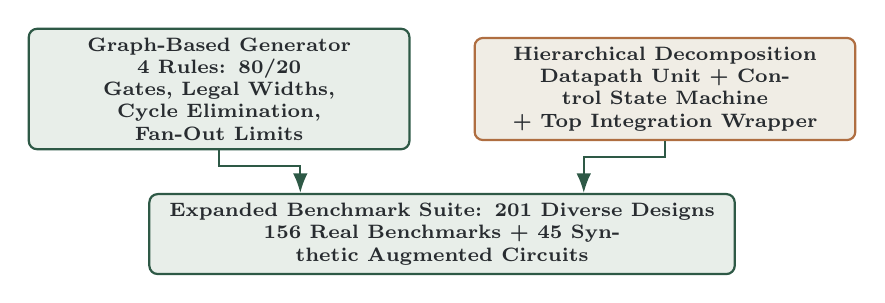
\begin{tikzpicture}[node distance=0.5cm and 0.8cm, auto]
        \node[block, text width=4.6cm] (rules) {Graph-Based Generator\\4 Rules: 80/20 Gates, Legal Widths,\\Cycle Elimination, Fan-Out Limits};
        \node[priorblock, text width=4.6cm, right=of rules] (hier) {Hierarchical Decomposition\\Datapath Unit + Control State Machine\\+ Top Integration Wrapper};
        \node[block, text width=7.2cm, below=0.6cm of $(rules.south)!0.5!(hier.south)$] (ds) {Expanded Benchmark Suite: 201 Diverse Designs\\156 Real Benchmarks + 45 Synthetic Augmented Circuits};

        \draw[arrow] (rules.south) -- ++(0,-0.2) -| ([xshift=-1.8cm]ds.north);
        \draw[arrow] (hier.south) -- ++(0,-0.2) -| ([xshift=1.8cm]ds.north);
    \end{tikzpicture}

    \vspace{0.3cm}
    \begin{block}{\centering Overcoming Data Scarcity}
        \centering\footnotesize
        Synthesizes fully legal, synthesizable hardware circuits across 5 diverse functional domains: Cryptography, DSP/FIR, Arithmetic, Control FSMs, and Memory.
    \end{block}
\end{frame}

% -------------------------------------------------------------
% Slide 12: Technology Transfer & Data Efficiency (Graph 3)
% -------------------------------------------------------------
\begin{frame}{Technology Transfer \& Data Efficiency}
    \begin{columns}[c]
        \begin{column}{0.60\textwidth}
            \centering
            \includegraphics[width=\textwidth,height=0.70\textheight,keepaspectratio]{fig14_augmentation_impact.png}
        \end{column}
        \begin{column}{0.38\textwidth}
            \begin{block}{\centering Robustness Insights}
                \footnotesize
                \begin{itemize}
                    \item Stable transfer across process operating corners (typical, fast, slow).
                    \item \textbf{Without Augmentation}: Accuracy collapses when real data is reduced.
                    \item \textbf{With Augmentation}: Retains \textbf{$R > 0.90$} even with a \textbf{60\% reduction} in real designs.
                \end{itemize}
            \end{block}
        \end{column}
    \end{columns}
\end{frame}

% -------------------------------------------------------------
% Slide 13: Numerical Comparison: Original Paper vs. Ours
% -------------------------------------------------------------
\begin{frame}{Numerical Comparison: Original Paper vs. Ours}
    10-Fold cross-validation results across all 201 designs:
    \vspace{0.3cm}
    \begin{table}[h]
        \centering\small
        \begin{tabular}{lcccc}
            \toprule
            \textbf{Target Metric} & \textbf{Original Paper Arch} & \textbf{Our Upgraded Arch} & \textbf{Improvement} \\
            \midrule
            \textbf{Area Error (MAPE)} & 5.21\% & \textbf{1.80\%} & \textbf{65\% Error Drop} \\
            \textbf{Area Correlation ($R$)} & 0.98 & \textbf{1.00} & Perfect Fidelity \\
            \midrule
            \textbf{Timing TNS ($R$)} & 0.90 & \textbf{0.97} & \textbf{+0.07 Correlation} \\
            \textbf{Timing WNS ($R$)} & 0.96 & \textbf{0.99} & \textbf{+0.03 Correlation} \\
            \midrule
            \textbf{Power Error (MAPE)} & 11.91\% & \textbf{10.14\%} & \textbf{15\% Error Drop} \\
            \textbf{Power Correlation ($R$)} & 0.95 & \textbf{0.97} & Consistent Scaling \\
            \bottomrule
        \end{tabular}
    \end{table}
\end{frame}

% -------------------------------------------------------------
% Slide 14: Things That Can Be Improved
% -------------------------------------------------------------
\begin{frame}{Things That Can Be Improved}
    \vspace{0.6cm}
    \begin{itemize}\setlength{\itemsep}{18pt}
        \item \textbf{Physical Wire Routing Congestion}:
        Moving beyond analytical fan-out RC approximations by integrating post-placement routing congestion maps.
        
        \item \textbf{Advanced Sub-7nm FinFET / GAA Nodes}:
        Expanding technology transfer models to sub-7nm process nodes with multi-corner multi-mode (MCMM) timing analysis.
        
        \item \textbf{Embedded SRAM and Memory Macros}:
        Extending standard-cell logic models to support large SRAM arrays and memory compilers for full-SoC chip estimation.
    \end{itemize}
\end{frame}

% -------------------------------------------------------------
% Slide 15: Summary & Key Takeaways
% -------------------------------------------------------------
\begin{frame}{Summary \& Key Takeaways}
    \begin{itemize}\setlength{\itemsep}{12pt}
        \item \textbf{Sub-Second Presynthesis Feedback}: Replaces hours of synthesis with millisecond ML inference.
        \item \textbf{Hybrid Physics Priors}: Combining circuit equations with gradient boosted residuals drops area error to \textbf{1.80\%}.
        \item \textbf{Outperforms Paper Baseline}: Consistently higher correlation across Area, Timing, and Power.
        \item \textbf{Scalable \& Robust}: Maintains high accuracy under severe training data scarcity.
    \end{itemize}
    \vfill
    \begin{center}
        \textbf{\color{SageGreen}Thank You!} \hspace{0.5cm} Questions \& Discussion
    \end{center}
\end{frame}

\end{document}
